\chapter{Predictive Modeling}

\section{Regression}

\subsubsection*{Statistical Models}

Statistical models are simplified descriptions of data that involve
mathematical relationships. In addition to the data itself,
a statistical model consists of \begin{inparaenum}[1)] \item a formula
  that specifies the mathematical relationships among the variables,
  and \item a description of how well the data agree with the model.
  \end{inparaenum} 
  Let's start with an example of how model formulas are represented in
  the R programming language. Recall the data set from
  Chapter~\ref{data-analysis} on speed, gender, and height for a
  sample of college students. Do we really think that, on average,
  males drive faster than females (or vice versa)? Similarly, is there
  any relationship between height and speed? The model formula is
\begin{Verbatim}
speed ~ height + gender
\end{Verbatim}
You should read the
formula above as ``Speed is modeled as a linear function of height and gender''.
The term to the left of the ``\mtilde'' is the
response or dependent variable and the terms to the right of the ``\mtilde''
that are separated by a ``\texttt{+}'' are the predictors or independent variables.
Mathematically, the formula
above specifies the model
\[
  speed_i = \beta_0 + \beta_1 height_i + \beta_2 gender_i + \epsilon_i
\]
where the coefficients $\beta_0,~\beta_1,~\beta_2$  along with the variance $\sigma_{\epsilon}^2$ of
the error term $\epsilon$ are the parameters to be estimated from the data.
The index $i$ refers to the $i$th observation in the data set.
Notice that neither the coefficients nor the error term appear in the R formula.
They are inferred and so we do not need to enter them. In particular
the R formula does not include the intercept term $\beta_0$. It is there
by default; this is usually what we want. The formula above is equivalent to
\begin{Verbatim}
speed ~ 1 + height + gender
\end{Verbatim}
If we do not want an intercept term in our model, say because we want to
force the fit to go through the origin, then we need to explicitly remove
the intercept, like this:
\begin{Verbatim}
speed ~ -1 + height + gender
\end{Verbatim}

Statistical modeling is a process that almost always involves iterating
over the following steps~\cite{chambers:1992}.
\begin{itemize}
\item obtaining data 
\item choosing a candidate model 
\item fitting the model, i.e. using software to  estimate the model parameters
\item interpretation of the fitted model parameters
\item diagnostics to see in what ways the model \emph{fails} to fit the data
\end{itemize}

\begin{comment}

The automobile data is available as a data frame that comes with
the \texttt{rpart} package. 
If you don't already have this package installed, then
\begin{Verbatim}
install.packages(``rpart'')
library(rpart)
attach(car.test.frame)
\end{Verbatim}
Having the data and a candidate model, let's fit the model
and plot \texttt{Mileage} against the values predicted by the model.
\begin{Verbatim}[samepage=true]
fm <- lm(Mileage ~ Weight + Disp.)
plot(fitted(fm), Mileage)
abline(0, 1, lty=2)
\end{Verbatim}
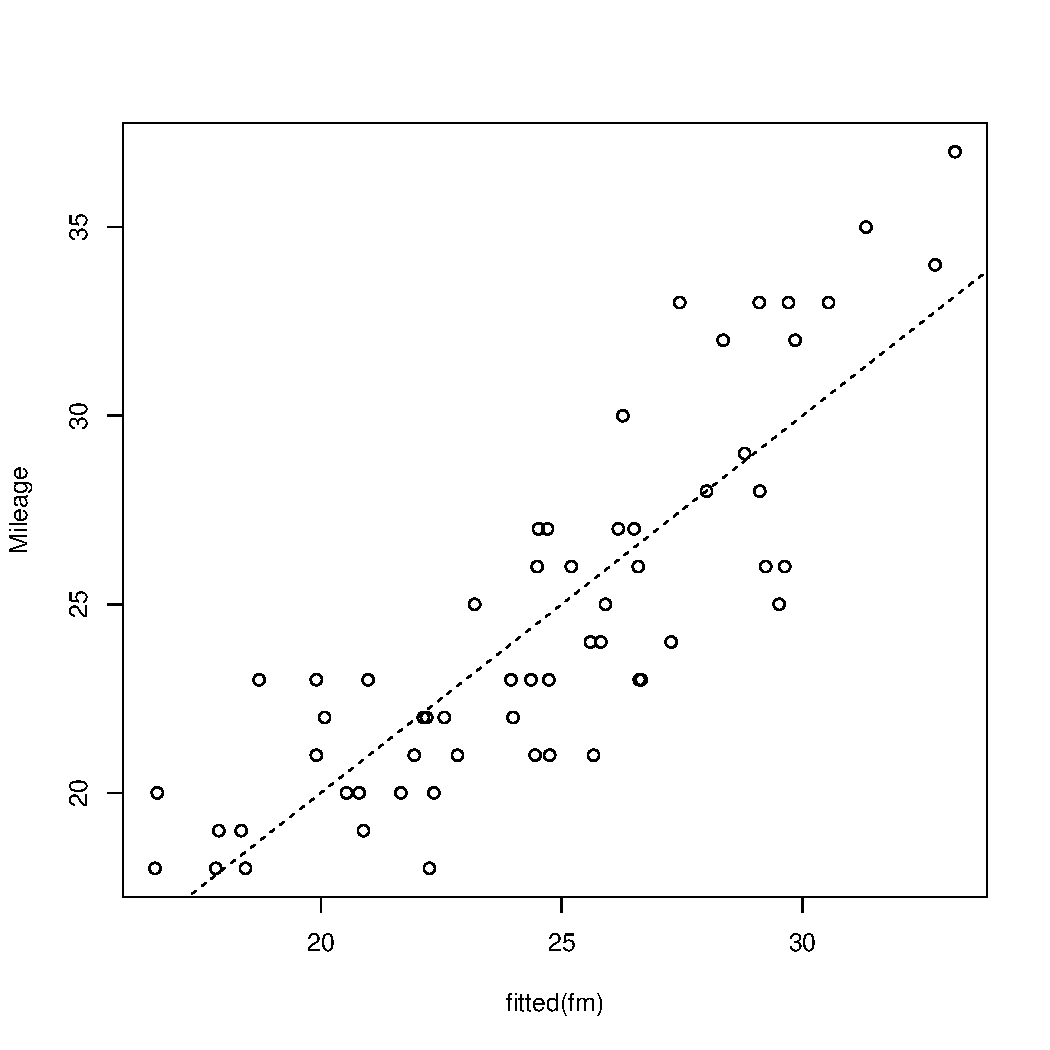
\includegraphics[width=0.7\textwidth]{Mileage-vs-fitted.pdf}

The dashed line in the plot represents a perfect fit. Qualitatively,
the model is doing pretty well, except for cars with high gas mileage.
Those points fall above the dashed line, an indication that the
predictions are too low. Let's try two different ways to improve the model,
1) by adding additional predictor variables to the model, and 2)
by changing our concept of how the data generating process should
be modeled. For example, let's suppose that we know something about
the physics of internal combustion engines in automobiles. Consequently,
we feel that fuel consumption is more natural than mileage as a
variable to relate linearly to weight. Noting that \texttt{Mileage}
is in units of miles per gallon, we can define fuel consumption in gallons per
100 miles driven as
\begin{Verbatim}
Fuel <- 100/Mileage
\end{Verbatim}
In other words, we want to try using the inverse of mileage as the
response variable.

\begin{enumerate}
\item Fit a model with \texttt{Mileage} as the response and
  \texttt{Weight}, \texttt{Disp.}, and \texttt{Type} as predictors.
  \texttt{Type} is a categorical variable with six levels: Compact,
  Large, Medium, Small, Sporty, and Van.
  Plot \texttt{Mileage} vs the fitted values. How does this model
  compare to the initial model?
\item Fit a model with \texttt{Fuel} as the response and
  \texttt{Weight} and \texttt{Disp.} as the predictors.  Plot
  \texttt{Fuel} vs the fitted values.  How does this model compare
  to the initial model?
\end{enumerate}

\end{comment}

% change this section into a discussion.
% it will come later in the section.
\subsubsection*{Transformations on Data}
  Suppose that a variable $u$ is related to a variable $v$ as
\[
u = \gamma_0e^{\gamma_1v}
\]
where $\gamma_0$ and $\gamma_1$ are parameters to be estimated.  Even
though the relationship between $u$ and $v$ is nonlinear, explain how
you could use simple linear regression to find estimates for
$\gamma_0$ and $\gamma_1$.

We can transform the relationship into a linear one
by taking logarithms.
\[
\text{ln}(u) = \text{ln}(\gamma_0) + \gamma_1v
\]
Then we have the form of a linear regression model with $\beta_0 = \text{ln}(\gamma_0)$
and $\beta_1 = \gamma_1$. After fitting the linear model,
\[
\hat{\gamma_0}=e^{\hat{\beta_0}}, \qquad \hat{\gamma_1} = \hat{\beta_1}
\]

% possible example to use
\begin{Verbatim}
## example of linear regression on the msleep data to
## notice that collinearity is present,
## choose variable transformation,
## understand the reported p-values,
## and understand the reported R-squared.
attach(msleep)

fm <- lm(sleep_total ~ brainwt + bodywt)
summary(fm)
## collinearity is present
plot(brainwt, bodywt)
plot(log(brainwt), log(bodywt))
fm <- lm(sleep_total ~ log(brainwt))
summary(fm)

## a one-unit increase in log(brainwt) decreases
## sleep time by about one hour (on avg).

## for interpretation, plug in a few values to get an idea
(x <- seq(from=0.5, to=5, by=0.5))
y.hat <- predict(fm, newdata=data.frame(brainwt=x))
plot(x, y.hat)

## the hypothesis test for b1

(t0 <- -1.0397/0.1914) # the t-statistic

pt(-5.432, 54) * 2  # the p-value
## should match the summary output

## compute R-squared
y.hat <- predict(fm)
y <- sleep_total[ !is.na(sleep_total) & !is.na(brainwt) ]

TSS <- sum( (y - mean(y))^2 )
RSS <- sum( (y - y.hat)^2 )
1 - RSS/TSS   # R-squared

(F <- ((TSS-RSS)/1) / (RSS/(56-1-1))) # the F-statistic
1 - pf(29.51, 1, 54)   # p-value for the F-test
\end{Verbatim}

\section{Classification}

\section{Time Series}

\section{Exercises}

\begin{enumerate}

\subsubsection*{Regression}
  
% this problem is OK
\item \emph{Old Faithful.}
In the \texttt{datasets} package in R there is a data set named
\text{faithful} that
contains data on the Old Faithful geyser in Yellowstone National Park,
Wyoming, USA.  The variables in the data set are
\begin{compactitem}[$\circ$]
\item \texttt{eruptions} the eruption time in minutes
\item \texttt{waiting} the time in minutes until the next eruption
\end{compactitem}

To view information about the data set, type
\begin{Verbatim}
> ?faithful
\end{Verbatim}
at the R prompt. Use this data to perform the following exercises.

\begin{enumerate}
\item Create histograms of \texttt{eruptions} and \texttt{waiting}
  (separately). \label{hist}

\item Create a scatter plot (i.e. an x--y plot) with \texttt{eruptions}
  on the x axis and \texttt{waiting} on the y axis. \label{scat}

\item From the histograms and the scatter plot that you created, what
  can you say about the behavior of the Old Faithful geyser? \label{interp}
  
\item Fit a linear regression model using the \texttt{lm()} function
  with \texttt{waiting} as the response variable and \texttt{eruptions}
  as the only predictor variable. Print a summary of the results.
  \begin{enumerate}
  \item What is the interpretation of the intercept? \label{int}
  \item What is your interpretation of the fitted coefficient
    on \texttt{eruptions}? \label{dur}

  \item You just observed an eruption of duration 4 minutes.
    Make a prediction on how long you will have to wait until
    the next eruption. Can you make any statement about the
    uncertainty in your prediction? In other words, can
    you give a range for the time until the next eruption?
    Don't worry about being exact with your range, just
    give something reasonable. \label{pred}.
  \end{enumerate}
\end{enumerate}

% this problem needs to be re-written.
% the questions are good, but we cannot use this data set.
\item \emph{VO2 max.} VO2 max is a measurement of the maximum amount
  of oxygen a person can utilize during intense exercise. The file
\texttt{vo2max-aerobic-fitness.csv} contains 20 observations of
VO2 max for people of various ages.
\begin{enumerate}
\item Fit a regression model with VO2 max as the response
variable and age as the predictor variable.
\item Plot the data and overlay the fitted regression line.
\item Provide an interpretation for the coefficient on age.
\item In your own words, state your interpretation of the $p$-value
for the coefficient on age.
\end{enumerate}
  
% written by braeden
\item \emph{Fuel efficiency.}
  For this problem we will be using a dataset called \texttt{mtcars}
  from the \texttt{datasets} package in R. This dataset contains data
  about different types of cars.  Fit a linear regression model using
  \texttt{lm()} with miles per gallon (\texttt{mpg}) as the response
  variable and the following predictor variables:
  \begin{compactitem}
  \item number of cylinders (\texttt{cyl})
  \item horsepower (\texttt{hp})
  \item weight in thousands of lbs (\texttt{wt})
    \end{compactitem}
    So the model is
    \[ mpg_i = \beta_0 + \beta_1 cyl_i + \beta_2 hp_i +
      \beta_3 wt_i + \epsilon_i \]
    Now do the following.
    \begin{enumerate}
    \item Looking at the summary of the fitted model, the coefficient for weight 
      $\beta_3 \approx -3.17$. What is the interpretation of $\beta_3$?
      
    \item How do the number of cylinders and horsepower affect fuel
      efficiency?
     
    \item Plot \texttt{mpg} as a function of
    \texttt{wt}. Overlay a fitted regression line from the
    full model onto the plot.  When plotting the regression line you
    should show \texttt{mpg} at the average \texttt{cyl} and average \texttt{hp}.
    In other words, it's a two-dimensional plot, but for the other
    variables that are not shown, we compute \texttt{mpg} at their
    average values. So you want to overlay
    \[ mpg_i = \beta_0 + \beta_1 \overline{cyl} +
      \beta_2 \overline{hp} +
      \beta_3 wt_i \]
    onto the data. You can use \texttt{coef()} to extract the
    coefficients from the fitted model object.

  \item Plot the actual \texttt{mpg} vs. the predicted (fitted)
    mpg. If your fitted model is stored in an object named
    \texttt{fm}, then you can get the predicted price as follows.
    \begin{Verbatim}
      mtcars$pred <- fitted(fm)
    \end{Verbatim}
    % $
    or
    \begin{Verbatim}
      mtcars$pred <- predict(fm)
    \end{Verbatim}
    % $

  \item In the summary output of the fitted model, the estimated residual
    standard error is reported to be
    $\hat{\sigma}_{\epsilon}=2.512$. Independently compute this quantity. In
    other words, use the actual values from the data and the fitted
    values from the model to compute the residual standard error
    yourself.  The formula is
    \[ \hat{\sigma}_{\epsilon} = \sqrt{ \frac{\sum_{i=1}^n \left(y_i - \hat{y_i}\right)^2}{n-k}} \]
    where $y_i$ and $\hat{y_i}$ are the actual and fitted values of observation
    $i$, respectively, $n$ is the total number of observations, and $k$ is the
    number of fitted parameters in the model. $n-k$ is the degrees of freedom.

  \item Do you think that a linear model is appropriate for this data?
  \end{enumerate}

% i'm not yet sure what i want to do with this problem.
\item \emph{Linear regression with numeric and categorical predictors.}
  The following sales data were
  collected for one particular product from a company for the past 10
  seasons.  The data are the price of the product that the company
  itself charged, the price that its competitor charged (for the
  competitor's version of the same product), the corresponding sales
  of the company's product, and the season. This data is available
  in the file \texttt{sales.csv}.

\begin{center}
\begin{tabular}{rrrl}
company price & competitor price & sales (1000s) & season \\ \hline
         \$10.2         &     \$9.9  &71.1 &winter \\
         11.6         &     9.9  &63.0 &summer \\
          9.8         &    11.7  &71.7 &winter \\
         13.7         &     9.5  &58.3 &summer \\
         12.0         &     8.9  &61.8 &summer \\
         11.2         &    10.1  &66.0 &summer \\
         10.2         &    11.1  &71.2 &winter \\
         10.6         &    10.7  &66.9 &winter \\
          9.5         &    12.6  &72.5 &winter \\
         11.8         &    10.0  &65.4 &winter
\end{tabular}
\end{center}

\begin{enumerate}
\item Create a visualization that shows all of the data on one plot.
  One idea is to plot sales vs. price, distinguish company and competitor
  price by symbol shape, and distinguish season by color.
  \item Fit a linear regression model 
\[
y = \beta_0 + \beta_1x_1 + \beta_2x_2 + \beta_3x_3
\]
where $y$ represents the sales in 1000s of units, $x_1$ represents
the company price in dollars, $x_2$ represents the competitor price in
dollars, and $x_3$ is an indicator variable as follows
\[
x_3 = \begin{cases} 0 \quad \text{if season is winter} \\
1 \quad \text{if season is summer}
\end{cases}
\]
\item Provide an interpretation each of the fitted parameters $\beta_0$, $\beta_1$,
  $\beta_2$, and $\beta_3$. \label{aa}
\item Do you think that competitor price should be included in the
  model?  Explain the reasoning for your answer. \label{bb}
\item What is the expected company sales if the company and the
  competitor both set their prices to \$11 for the winter season?  Use
  the full model, regardless of your answer to
  part~\ref{bb} \label{cc}
\end{enumerate}

% I need to check if this problem needs to be re-written.  The data is
% from harrell's book, but we may be able to use it. the idea is to
% fit a logistic regression model with one numeric predictor and one
% categorical predictor and view the response on the probability scale
% graphically.
\item \emph{Logistic regression.} The file \texttt{harrell.csv}
contains data on 40 people. The variables are \texttt{age} in years,
\texttt{gender}, a categorical variable with two levels, \texttt{female}
and \texttt{male}, and \texttt{response}, a 0/1 indicator variable for
whether the person responded to a medical treatment (1 means that the
person responded). Fit a logistic regression model with
\texttt{response} as the dependent variable and \texttt{age} and
\texttt{gender} as the independent variables.

\begin{enumerate}
\item How does the probability of response change for a 42-year-old male
compared to a 52-year-old male?
\item Which gender has a higher probability of response to the medical
treatment?
\item What is the effect on the odds of response for a one--year
increase in age?
\item Make a plot of the probability of response as a function
of age, with one curve for females and one curve for males.
\end{enumerate}

\subsubsection*{Classification}

\subsubsection*{Time Series}

\item \emph{Simulation of a simple trading strategy.}
  The file \texttt{BTC-USD.csv} contains one year's worth of price
  data on Bitcoin. The \texttt{Close} column is the price of
  Bitcoin in USD on \texttt{Date}. 

\begin{enumerate}
\item Read the data into an R data frame.
\item Turn the \texttt{Date} field into a proper Date variable rather
  than a character string.
\item Make a time-series plot with \texttt{Date} on the x axis and
  \texttt{Close} on the y axis.
\item Make a scatter plot with \texttt{Volume} on the x axis and
  \texttt{Close} on the y axis. Do you see a pattern? Try making
  this plot using a logarithmic transformation on \texttt{Volume} and
  \texttt{Close}.
\item Create a one-step-ahead forecast for the closing price using
  simple exponential smoothing. Use a smoothing parameter value
  of $\alpha = 0.5$.
\item Using your forecast simulate a very simple trading strategy.
  The strategy is: if the forecast is for a price increase then buy,
  otherwise if the forecast is for a price decrease then sell. Don't
  worry about the bid/ask spread, trading fees, or any of the messy
  details. You are simply buying or selling one Bitcoin at the closing
  price. Keep track of your gain/loss. How did you do? Do you
  have any criticisms of this trading strategy?
\item  Now plot your forecasted/predicted price and the actual price
  on the same plot. Do you see a general behavior in the forecast?
  Experiment with different values for $\alpha$.
\end{enumerate}
  
\end{enumerate}
